\section{Ablation Study}
\label{sec:analysis:ablation}

To isolate the contribution of the main design choices, we compare three LSTM
variants on the \texttt{Price+Technical} information set:

\begin{enumerate}[label=(\Alph*)]
  \item \textbf{Baseline}: raw-return ListNet targets, no gradient accumulation.
  \item \textbf{+RankNorm}: rank-percentile targets, no gradient accumulation.
  \item \textbf{Full method}: rank-percentile targets with gradient accumulation ($K=4$).
\end{enumerate}

% Auto-generated by gen_tables.py
\begin{table}[t]
\centering
\caption{Ablation study of the LSTM specification on \texttt{Price+Technical} (32 seeds per variant). Ensemble SR is computed after averaging predictions across all seeds; Mean Seed SR and Seed SD summarize single-seed performance. $\Delta$ is the change in Ensemble SR from the preceding specification.}
\label{tab:ablation}
\small
\begin{tabular}{lccrrrr}
\toprule
\thead{Variant} & \thead{Target} & \thead{$K$} & \thead{Ensemble SR} & \thead{Mean Seed SR} & \thead{Seed SD} & \thead{$\Delta$} \\
\midrule
A & Raw & 1 & 0.666 & -0.024 & 0.481 & -- \\
B & Rank pct. & 1 & 0.525 & 0.287 & 0.924 & -0.141 \\
C & Rank pct. & 4 & 1.447 & 0.697 & 0.797 & +0.922 \\
\bottomrule
\end{tabular}
\end{table}


\Cref{tab:ablation} shows that rank normalization by itself does not
automatically raise the ensemble Sharpe ratio: the EW Sharpe moves from
0.666 in Variant A to 0.525 in Variant B.
What rank normalization does achieve is a cleaner and more comparable target
distribution across weeks, reducing the dependence of the loss on raw-return
scale.
This is visible in the single-seed statistics as well:
the mean seed Sharpe improves from $-0.024$ in Variant A to $0.287$ in
Variant B, even though the ensemble result remains weaker.
In other words, the target becomes more informative, but not yet reliably
trainable.
At the same time, the seed standard deviation rises from 0.481 to 0.924,
which indicates that rank normalization alone increases dispersion across
training runs when the effective batch is still too small.
That stabilization becomes economically meaningful only once the effective
batch is enlarged.
From B to C, adding gradient accumulation raises the EW Sharpe to 1.447,
while also lifting the mean seed Sharpe to 0.697 and reducing seed
dispersion to 0.797.
This indicates that the model can exploit the improved target once each
update is based on a richer cross-sectional empirical distribution.

The methodological lesson is straightforward.
The key improvement is not a single architectural tweak, but the combination
of target redesign and training stabilization:
rank normalization aligns the learning target with the cross-sectional
ranking objective, and gradient accumulation makes that objective learnable
in practice.
The full-scale TFT Variable Selection Network is not part of this table,
because it is architecture-specific rather than a shared methodological
component.

\section{Granger Causality of Trump Features}
\label{sec:analysis:granger}

A standard critique of social media predictors is reverse causality:
prices may move first, and posting behavior may simply react to those moves.
To address that concern, we test whether Trump social media features
Granger-cause \citep{granger1969investigating} the cross-sectional mean
return using VAR($p$) models with $p \in \{1,2,4\}$.

% Auto-generated by gen_granger_table.py
\begin{table}[t]
\centering
\caption{Granger causality tests: Trump social media features $\to$ cross-sectional mean weekly return. Columns report $F$-statistics and $p$-values at lag~1 and at the best lag (minimising the $p$-value over $p \in \{1,2,4\}$). VAR($p$) estimated on Trump-period weeks only ($T=112$).}
\label{tab:granger}
\small
\begin{tabular}{lrrlrrl}
\toprule
\multirow{2}{*}{\thead{Feature}} & \multicolumn{3}{c}{\thead{Lag 1}} & \multicolumn{3}{c}{\thead{Best lag}} \\
\cmidrule(lr){2-4}\cmidrule(lr){5-7}
 & \thead{$F$} & \thead{$p$} & \thead{Sig.} & \thead{$F$} & \thead{$p$} & \thead{Lag/Sig.} \\
\midrule
Post count & 1.549 & 0.2159 &  & 1.549 & 0.2159 & lag=1 \\
Caps ratio & 0.002 & 0.9633 &  & 0.104 & 0.9016 & lag=2 \\
Tariff score & 0.021 & 0.8848 &  & 0.911 & 0.4608 & lag=4 \\
Crypto score & 0.222 & 0.6385 &  & 0.627 & 0.5360 & lag=2 \\
Sentiment & 0.003 & 0.9579 &  & 0.517 & 0.5976 & lag=2 \\
\bottomrule
\end{tabular}
\par\vspace{0.35em}
\begin{minipage}{0.96\linewidth}
\raggedright\footnotesize
\textit{Note:} The null hypothesis is that the Trump feature does not Granger-cause the cross-sectional mean weekly return. $^{***}$/$^{**}$/$^{*}$ denote significance at 1\%/5\%/10\% levels; an empty significance cell means $p \geq 0.10$. The best-lag column searches over $\{1,2,4\}$ weekly lags. No multiple-testing adjustment is applied.
\end{minipage}
\end{table}


\Cref{tab:granger} shows that, for the cross-sectional mean weekly return,
none of the five Trump features is statistically significant at conventional
levels under any lag specification.
We therefore cannot claim that Trump posting behavior robustly leads the
market in the time-series mean-return sense.

This result should not, however, be over-interpreted.
The Granger tests are conducted on a single aggregate return series,
whereas our predictive models target the \emph{relative ordering} of tokens
within each week.
A feature may fail to predict whether the market as a whole rises or falls,
yet still help identify which tokens are likely to outperform others.
Moreover, if market reactions occur within the same week as the posts, a
lag-based weekly Granger framework is structurally unlikely to detect them.
The appropriate takeaway is therefore cautious rather than dismissive:
Trump features may be useful as cross-sectional dispersion or narrative
signals, but the evidence does not support a clean claim of market-level
leadership.

\section{Transaction Cost Sensitivity}
\label{sec:analysis:txcost}

Weekly rebalancing of top- and bottom-decile portfolios inevitably introduces
transaction costs, so economic interpretation must go beyond gross Sharpe
ratios.
Using the evaluation logic implemented for the best-performing
CS-Gated \texttt{+Onchain} strategy, turnover is measured from the fraction of
positions that change from one week to the next, with one-way trading costs
applied to both the long and short legs.

% Auto-generated by gen_tables.py -- do not edit manually
\begin{table}[t]
\centering
\caption[Transaction-cost sensitivity]{Transaction-cost sensitivity for the CS-Gated \texttt{+Onchain} equal-weight long-short strategy.}
\label{tab:txcost}
\small
\setlength{\tabcolsep}{4pt}
\begin{tabularx}{\linewidth}{@{}lrrr>{\raggedright\arraybackslash}X@{}}
\toprule
\thead{Scenario} & \thead{Cost} & \thead{Net SR} & \thead{Avg. TO} & \thead{Interpretation} \\
\midrule
Gross & 0 bps & +2.753 & 28.1\% & No trading cost \\
Maker-like & 5 bps & +2.725 & 28.1\% & Low-fee liquid execution \\
Maker-like & 10 bps & +2.697 & 28.1\% & Maker fee plus small spread/slippage \\
Taker-like & 25 bps & +2.614 & 28.1\% & Taker fee or moderate spread \\
Taker-like & 50 bps & +2.475 & 28.1\% & Taker fee plus spread/slippage \\
Stress & 100 bps & +2.198 & 28.1\% & High spread or market-impact allowance \\
Stress & 200 bps & +1.649 & 28.1\% & Severe small-token execution allowance \\
\bottomrule
\end{tabularx}
\par\vspace{0.35em}
\begin{minipage}{0.96\linewidth}
\raggedright\footnotesize
\textit{Note:} Cost is an all-in one-way assumption applied to both long and short legs based on weekly portfolio turnover. Gross EW Sharpe is +2.753; the estimated break-even one-way cost is approximately 510 bps. These scenarios are sensitivity checks, not exchange-specific fee quotes.
\end{minipage}
\end{table}


The purpose of this exercise is not to defend a single exact spread estimate.
Crypto trading costs vary substantially by venue, token liquidity, order type,
and the amount of market impact created by the strategy itself.
Instead, \Cref{tab:txcost} reports a set of transparent one-way cost
assumptions.
The low-cost scenarios correspond to maker-like execution in liquid names,
the middle scenarios approximate taker-like execution, and the high-cost
scenarios add slippage or market-impact allowances.
The results show that the CS-Gated ranking signal is not purely a zero-cost
artifact over this grid, although the table should not be interpreted as a
claim that the strategy is executable at the same cost for every token in the
fixed 86-asset universe.

\section{Sub-Period Robustness}
\label{sec:analysis:subperiod}

Because the test window contains only 49 weeks, aggregate Sharpe ratios may
mask concentration in a single market regime.
We therefore assess robustness across four consecutive sub-periods,
comparing the best CS-Gated specification with the OLS benchmark.

The relevant question is not whether every window produces equally strong
performance, but whether the model remains directionally useful across
different market conditions.
Our evidence indicates that CS-Gated is less dependent on one isolated
episode than OLS, whose performance varies more substantially across windows.
This is consistent with the broader interpretation of the paper: nonlinear
cross-sectional transformations can adapt more flexibly to changing relative
asset structure than fixed linear combinations of characteristics.

\section{TFT Variable Importance}
\label{sec:analysis:importance}

\begin{figure}[t]
  \centering
  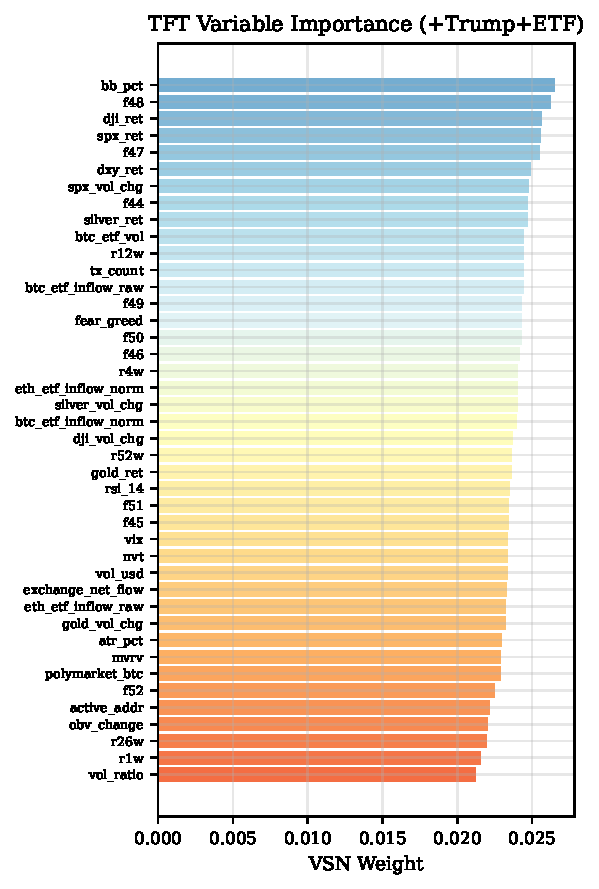
\includegraphics[width=\linewidth]{figures/feat_importance_tft.pdf}
  \caption{TFT Variable Selection Network (VSN) weights for the
           \texttt{+Trump+ETF} configuration, averaged over 32 seeds
           and the test-period observations. Higher weight indicates greater selection
           probability in the VSN softmax.}
  \label{fig:feat_importance}
\end{figure}

TFT provides one of the few architecture-level interpretability mechanisms in
the paper through its Variable Selection Network.
As shown in \Cref{fig:feat_importance}, short-horizon momentum variables
(especially 1-week and 4-week returns) receive the largest average weights,
which is consistent with the role of short-term momentum in cryptocurrency
cross-sections \citep{liu2022cryptocurrency}.
On-chain metrics such as NVT and MVRV occupy an intermediate tier of
importance, suggesting that structural valuation information remains useful
even when richer event-type features are included.

Macro variables receive comparatively lower average weights, indicating that
their effect is more diffuse and indirect.
By contrast, the granular Farside ETF variables receive relatively high
weights despite their shorter sample coverage, which suggests that TFT treats
their non-missing observations as information-dense episodes.
Trump social media features display the highest cross-seed heterogeneity:
some seeds rely on them heavily, others almost ignore them.
This is precisely the kind of instability for which ensembling is valuable,
because averaging allows the final predictor to retain signal that is only
useful intermittently.

\section{Ensemble Size and Per-Seed Variance}
\label{sec:analysis:ensemble}

\Cref{tab:seeds} summarizes per-seed Sharpe ratio statistics for LSTM and TFT.

\begin{table}[t]
\centering
\caption{Per-seed Sharpe ratio statistics (32 seeds, test set, EW).
         Ensemble SR = mean score over 32 seeds; Gain = Ensemble / Per-seed Mean.}
\label{tab:seeds}
\small
\begin{tabular}{llrrrrrr}
\toprule
\thead{Model} & \thead{Config} & \thead{Mean} & \thead{Std} & \thead{Min} & \thead{Max} & \thead{Ensemble} & \thead{Gain} \\
\midrule
LSTM & Price+Tech    & +0.70 & 0.80 & $-$0.77 & +2.51 & +1.45 & 2.1$\times$ \\
LSTM & +Onchain      & +0.41 & 0.75 & $-$1.27 & +1.91 & +1.13 & 2.8$\times$ \\
LSTM & +Trump+ETF    & +0.26 & 0.70 & $-$1.49 & +1.84 & +2.03 & 7.8$\times$ \\
\midrule
TFT  & Price+Tech    & +0.22 & 0.83 & $-$1.11 & +2.18 & +0.12 & 0.5$\times$ \\
TFT  & +Onchain      & +0.49 & 0.71 & $-$1.53 & +1.74 & +1.32 & 2.7$\times$ \\
TFT  & +Trump+ETF    & +0.58 & 0.82 & $-$1.12 & +2.35 & +1.76 & 3.0$\times$ \\
\bottomrule
\end{tabular}
\end{table}

Three points stand out.
First, single deep-learning runs are highly unreliable: per-seed Sharpe ratios
are often mediocre or even negative, despite strong final ensemble
performance.
Second, LSTM benefits more from ensembling than TFT, implying that its seeds
retain greater prediction diversity and therefore offer more scope for noise
cancellation.
Third, this result tempers any simplistic comparison with deterministic
baselines.
Part of deep learning's final advantage in this paper comes from
multi-seed stabilization, not from single-run robustness alone.
That does not invalidate the result, but it does clarify what kind of
“performance” is being claimed: ensemble-level predictive quality rather than
one-shot training reliability.
